\section{Features Common to Both Spectrometers}

\subsection{Vacuum Windows}

Because multiple scattering degrades the performance of a spectrometer, it is
important that the spectrometer volume be evacuated and that the vacuum
entrance and exit windows be as low mass as possible. However,
catastrophic window failure would generate a significant shock wave as air
rushed to fill the vacuum volume. It would also cause a loud noise which
could cause hearing damage to anyone in the immediate vicinity.
The material chosen for the vacuum windows, then, must be both light enough
to have a minimum effect on the beam and strong enough to operate reliably and safely.

{\bf One of the responsible personnel must be present for
any work directly affecting any Hall~C vacuum window}. Refer to Table ~\ref{tab:spectrometers:personnel_vacuum}.

Thin metal windows have an indefinite lifetime and cause
multiple scattering which is small compared to the intrinsic resolution of
the Hall-C spectrometers. Both the HMS and the SHMS are now equipped
with metal windows, as detailed in Table ~\ref{tab:hall_c_windows_specs}.

\begin{namestab}{tab:spectrometers:personnel_vacuum}{Spectrometer Vacuum: authorized personnel}{%
      List of Spectrometer Vacuum responsible personnel where ``W.B.'' stands for the white board
      in the counting house.}
   \TechonCall{\em Contact}
   \JerryNines{}
\end{namestab}

\begin{table}
\begin{center}
\caption{Vacuum Windows in Hall C\label{tab:hall_c_windows_specs}}
%\vspace{\baselineskip}
\begin{tabular}{|l|l|l|l|}
\hline
Window Location				& Dimensions (mm) 	 	& Material & Thickness (mm) \\ \hline
Scattering Chamber Exit			& Very Wide		& Al		& 0.406\\
HMS Entrance	on Snout			& 254  (dia)		& Al		& 0.508\\
HMS Exit						& 1016  (dia)		& Al		& 0.508\\
SHMS Entrance on HB Magnet		& $180(w) \times 220(h)$	& Al	& 0.508\\
SHMS Dipole Exit				& 692 (dia)		& Al		& 0.508\\
SHMS Exit from Vacuum Extension	& 692 (dia)		& Al		& 0.508\\
\hline
\end{tabular}
\end{center}
\end{table}

\subsubsection{HMS Windows}

The entrance window to the HMS vacuum channel is on the end of the
snout which extends from the HMS Q1 magnet towards the target.The vacuum
channel has a volume of approximately $6$ m$^3$, representing a stored energy of
$6 \times 10^5$~Joules. A drawing of the  flange to which the exit vacuum
window is attached is shown in Figure~\ref{fig:hms_flange}.  The window is a
circle that covers the $38$ inch diameter opening and has bolt holes for clamping
it in place along a $40$ inch center-to-center diameter.
This is the largest vacuum window in Hall~C. Under vacuum, it must support 16,785
lbs (74,425 N). It is located in the HMS detector hut as shown in Fig.~\ref{fig:hms_window2}.

To protect this window from damage, and for the safety of people working in the HMS
shield house, an aluminum shutter plate must be lowered to cover the HMS exit
window whenever it is under vacuum and the door to the detector hut is open.
A system of interlocks assures that these conditions are met. The shutter
control panel is just outside the shielding house door, and an
indicator light signals whether the shutter is in or out.  The shutter must be closed
before the shield house door may be opened. \emph{Note that the shutter needs to be
open when data is being taken by the HMS, and the shutter may be opened only
after the shield door is closed.}

\begin{figure}
\begin{center}
\includegraphics[width=4in]{figHMSflange}
\caption{The HMS Exit Window Flange and Vacuum Spool Piece. The opening covered
by the window is 38 inches in diameter. \label{fig:hms_flange}}
\end{center}
\end{figure}

\begin{figure}
\begin{center}
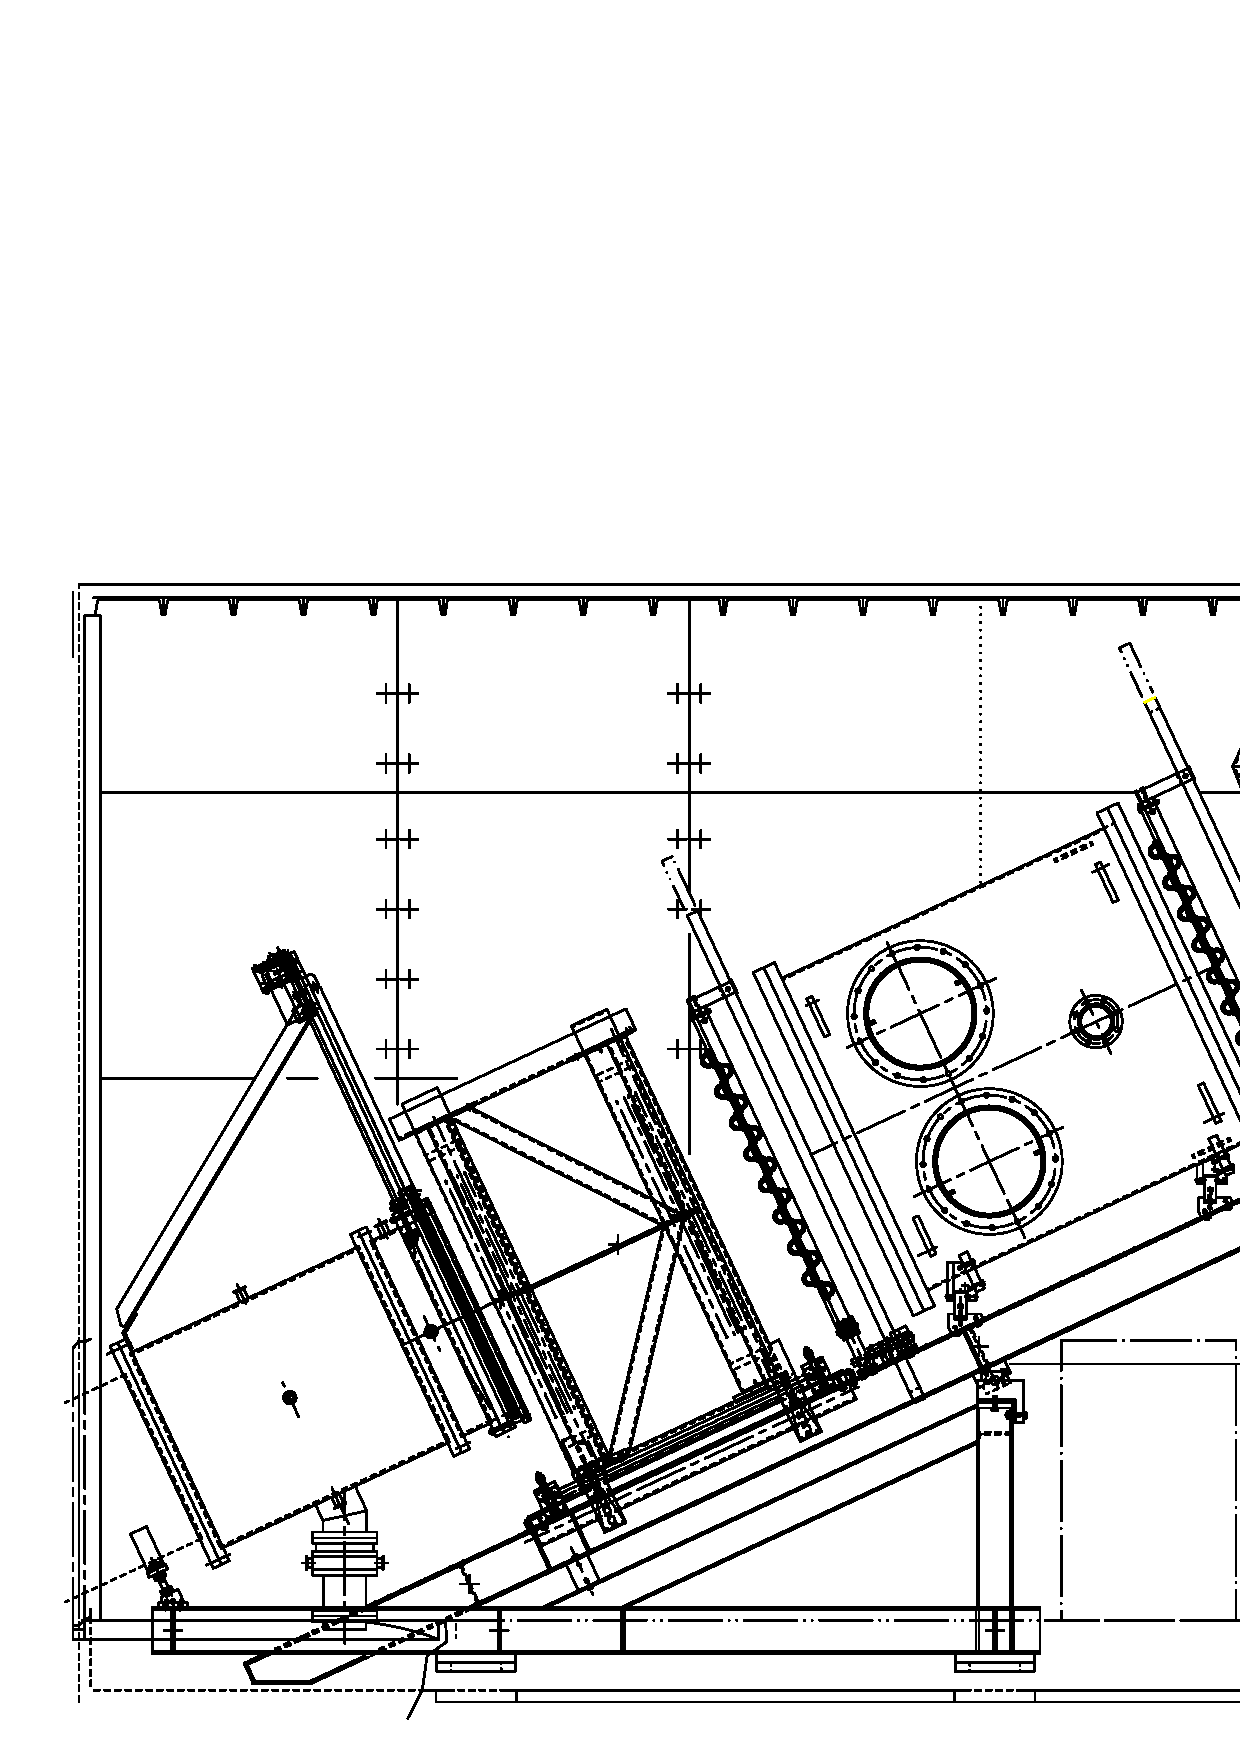
\includegraphics[width=4in]{figHMShut}
\caption{The HMS vacuum window in the HMS spectrometer hut.
\label{fig:hms_window2}}
\end{center}
\end{figure}

\subsubsection{SHMS Windows}
\label{sec:shmswindows}
The SHMS entrance window is on the front of the HB magnet. It has a rectangular shape.
The SHMS exit window is inside the Shield House detector room. It is mounted on the
downstream end of the SHMS dipole when the Noble Gas Cherenkov (NGC)
is in use. Otherwise, it is mounted on the vacuum extension tank.  These two locations
are indicated in Fig.~\ref{fig:shms_exit_window_locations}.  Drawings of
the window and its flanges are shown in Fig.~\ref{fig:shms_exit_window}. When in use
the NGC provides protection for the vacuum window. When the window is placed on
the end of the vacuum extension tank, however, it must be protected by a roll-down
shutter that is interlocked with the detector-room door: if the door is open the shutter
must be down, protecting the window. Just like the HMS, \emph{the shutter needs to be
open when data is being taken by the SHMS, and the shutter may be opened only
after the shield door is closed.} The SHMS shutter controls are to be located near
the ``barn door'' separating the SHMS detector shield house from the SHMS electronics
shield house and are described in section~\ref{sec:shmswindows}.

\begin{figure}
\begin{center}
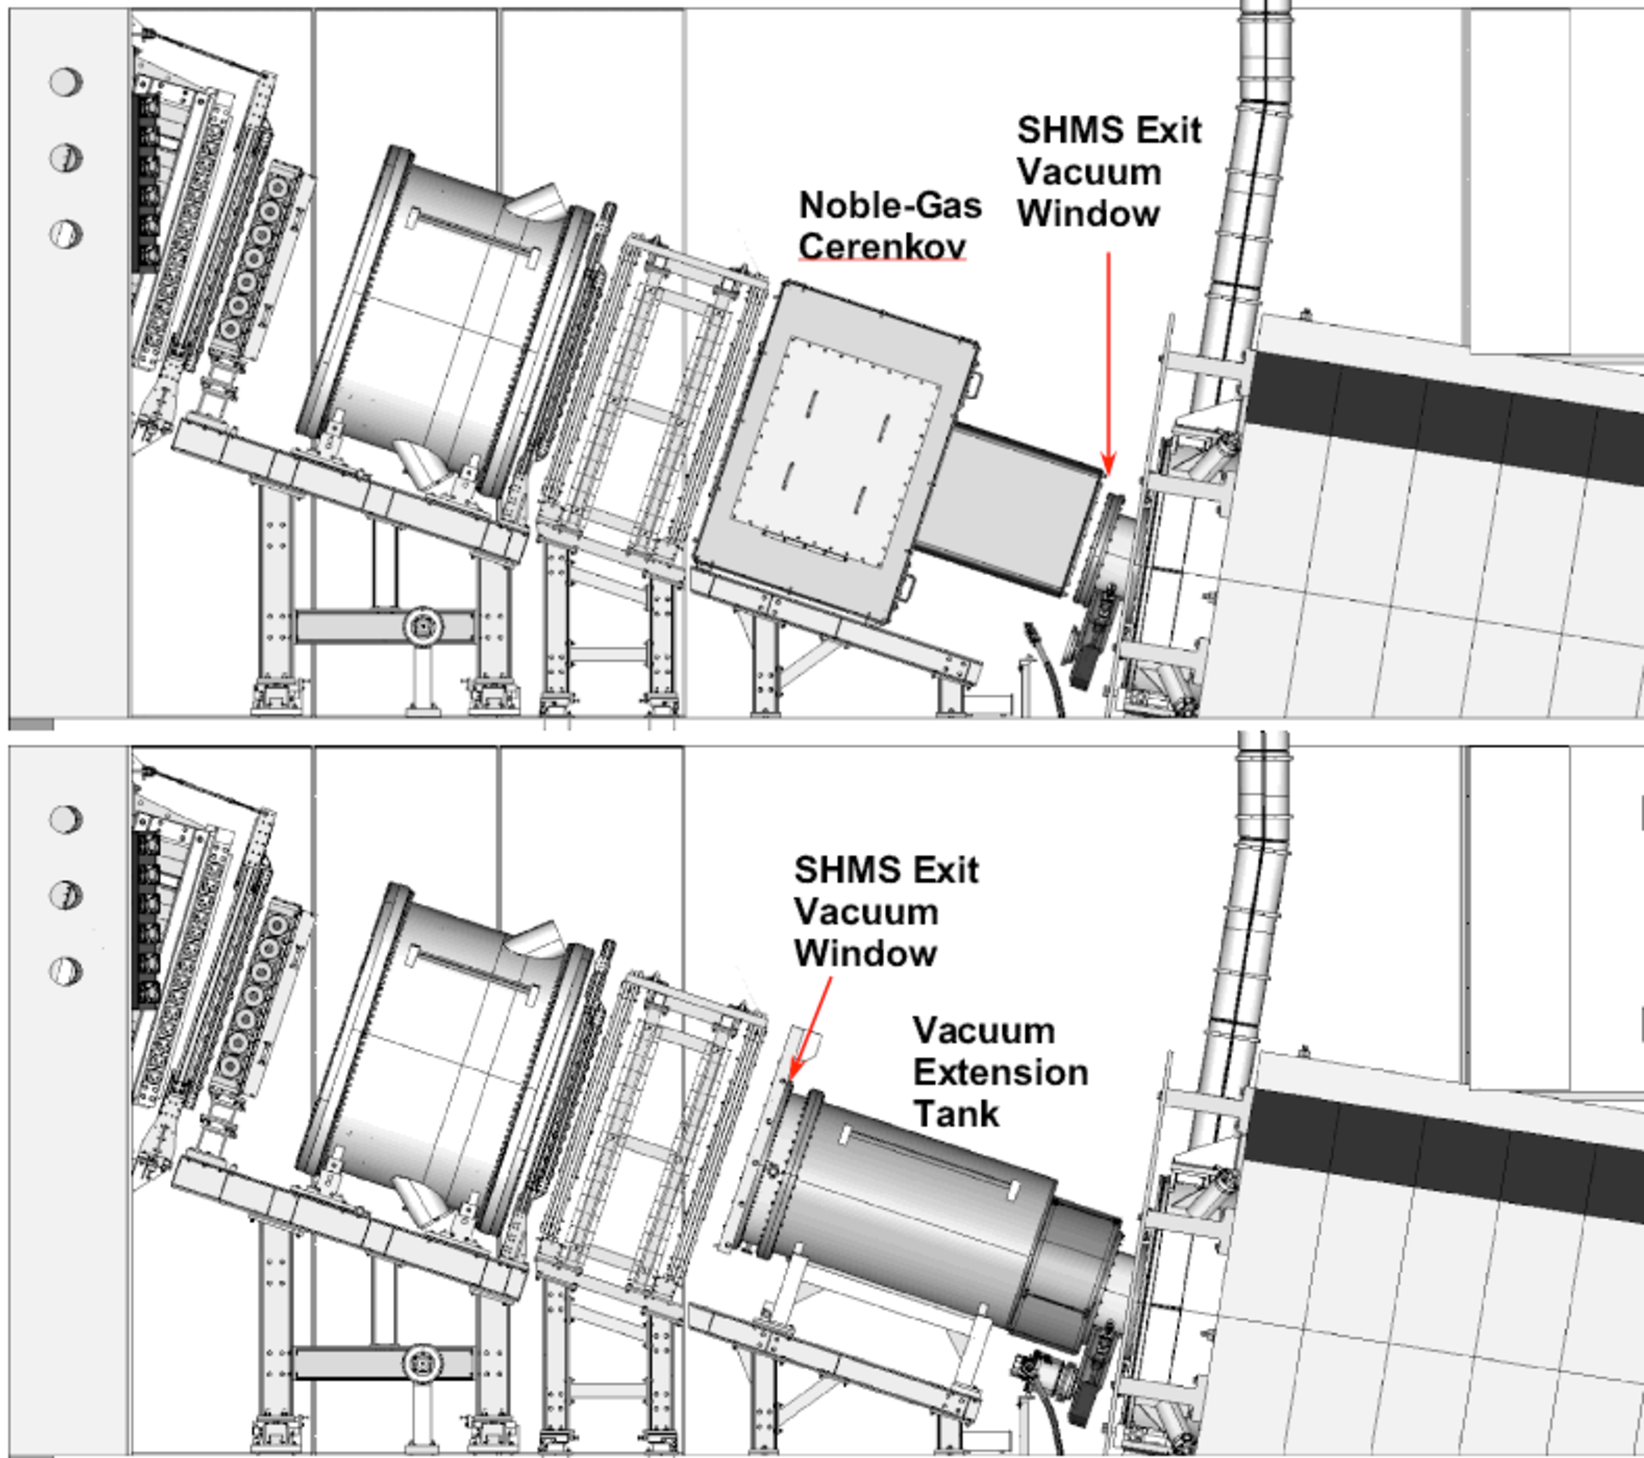
\includegraphics[width=6in]{figSHMS_ExitWindowLocations}
\caption{The two possible locations of the SHMS Exit Vacuum Window \label{fig:shms_exit_window_locations}}
\end{center}
\end{figure}

\begin{figure}
\begin{center}
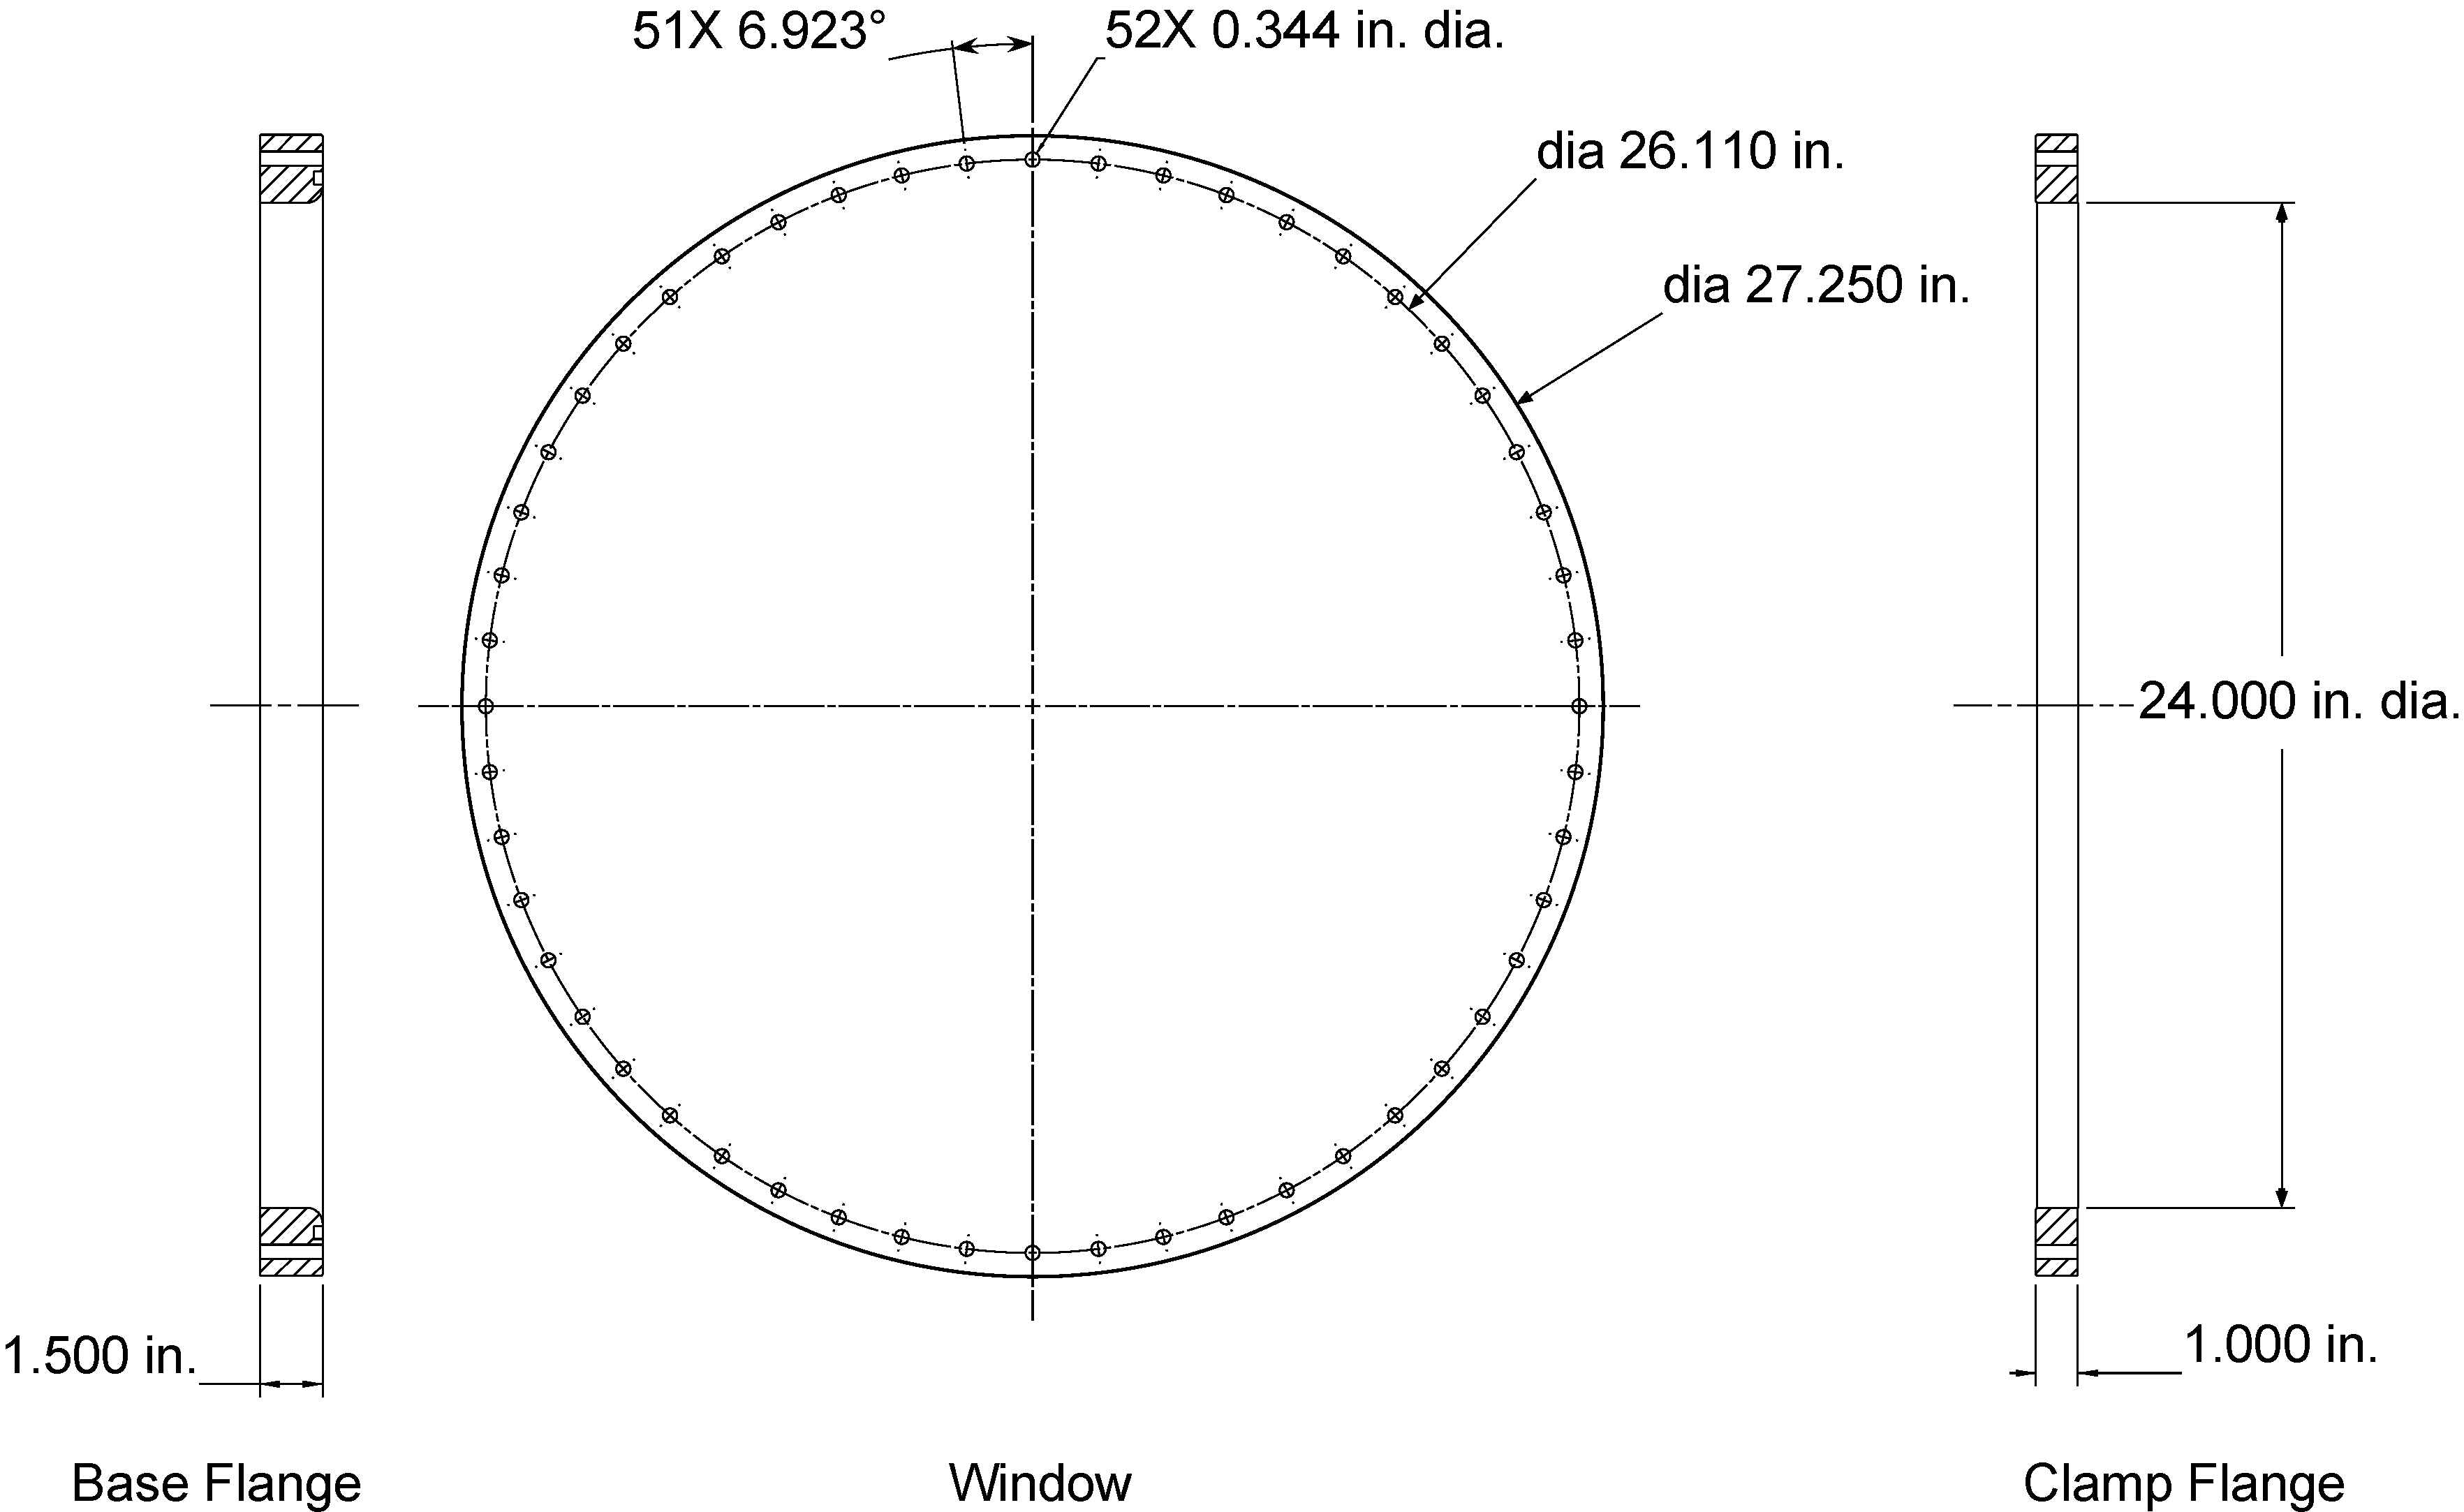
\includegraphics[width=4in]{figSHMSexitWindow}
\caption{The SHMS Exit Vacuum Window and Flange. \label{fig:shms_exit_window}}
\end{center}
\end{figure}
